

\section*{Task 5}

%\title{Introduction to \LaTeX{}}
%\author{Author's Name}
%\maketitle

%\begin{abstract}
%The abstract text goes here.
%\end{abstract}


\section{Two BCD addition}

\begin{figure}[H]
  \begin{centering}
  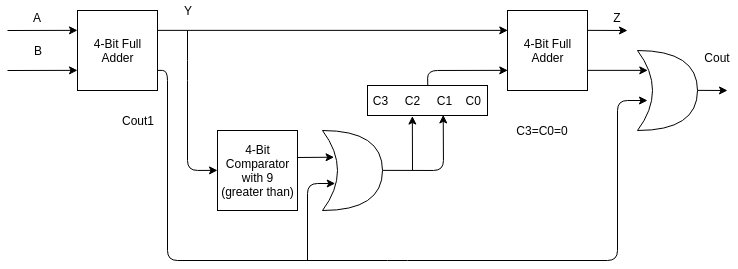
\includegraphics[scale=0.5]{data/ej5.png}
  \par\end{centering}
  \caption{Block diagram of the 4-Bit BCD sum}
\end{figure}
Given two numbers in BCD format, return the two-digits value of the sum of these two numbers.
In order to implement this task, two 4-bit Full Adders were instantiated from the same module.
Assuming that inputs are valid, there are just two cases to analyze. 
First of all, if the sum of the two numbers in decimal is greater than 9 or the carryout bit from the first Full Adder, the sum of them showed in binary code is not the actual BCD.   
To get the right answer it's necessary to add 6 in decimal value to the sum of those two numbers in order to get the BCD equivalent. Otherwise, there is not addition to the sum of those two numbers.


%\begin{equation}
%    \label{simple_equation}
%    \alpha = \sqrt{ \beta }
%\end{equation}

\subsection{Input}
Two BCD digits must be entered with the following format:
./a.out +a=XXXX +b=YYYY
Where a.out is the name of output executable and both XXXX and YYYY are two 4-bit binary numbers.
\subsection{Output}
The output number is shown as an 8-bit BCD format.

%\section{Conclusion}
%Write your conclusion here.
